\documentclass[11pt]{article}
\usepackage{qftnotes}
\usepackage{tikz}

\title{Phase 0 $\cdot$ Classical Mechanics --- Lesson 2:\\ Hamiltonians and Poisson Brackets}
\author{Self-study companion to \emph{Quantum Field Theory for the Gifted Amateur}}
\date{}

\newcommand{\hb}{\hbar}
\newcommand{\hatq}{\hat q}

\begin{document}
\maketitle
\vspace{-2em}

\begin{tcolorbox}[colback=gray!6,colframe=gray!50!black,title={Lesson at a glance},fonttitle=\bfseries]
\textbf{Prerequisites.} Lesson 1 (action, Euler--Lagrange equations, the Klein--Gordon Lagrangian density); multivariable calculus; the idea of a delta function.

\textbf{Time estimate.} About 2--3 hours, plus time for the exercises.

\textbf{Learning goals.} By the end you should be able to:
\begin{itemize}[nosep]
  \item compute canonical momenta and pass from $L$ to $H$ by a Legendre transform, and derive Hamilton's equations in two ways;
  \item picture motion as flow in phase space;
  \item use Poisson brackets to compute time evolution and to identify conserved quantities;
  \item recognise canonical transformations, and see the harmonic oscillator's ladder variables $a,a^*$ emerge classically;
  \item state Dirac's rule $\{A,B\}\to \frac{1}{i\hbar}[\hat A,\hat B]$;
  \item write down $\pi$ and $\Ham$ for a classical field and see why $[\hat\phi(\vect x),\hat\pi(\vect y)]=i\delta^3(\vect x-\vect y)$ is the natural quantum condition.
\end{itemize}
\end{tcolorbox}

\tableofcontents
\bigskip

%=====================================================================
\section{Why the Hamiltonian?}

In Lesson 1 we built mechanics on the action: the Lagrangian $L(q,\dot q,t)$ is the primary object, and the equations of motion are the Euler--Lagrange equations. That formulation is elegant and, as we shall see in Lesson 3, makes symmetries transparent. But quantum mechanics is not built on the Lagrangian. It is built on the \emph{Hamiltonian}: the time-dependent Schr\"odinger equation is $i\hbar\,\partial_t\psi=\hat H\psi$, and the Heisenberg equation of motion is $\dot{\hat A}=\frac1{i\hbar}[\hat A,\hat H]$.

The bridge between the classical and quantum worlds is therefore a classical reformulation that looks as much as possible like the quantum one. The Hamiltonian formulation provides exactly this. Its punchline, which we will arrive at in Section~\ref{sec:dirac}, is a recipe:
\[
 \text{classical Poisson bracket}\ \pb{A}{B}\quad\longrightarrow\quad \text{commutator}\ \tfrac{1}{i\hbar}\comm{\hat A}{\hat B}.
\]
This is \emph{canonical quantization}, and it is precisely how Lancaster \& Blundell (L\&B) quantize the harmonic oscillator and, later, the scalar field.

\begin{qftbridge}
Everything in this lesson is used again in L\&B. The oscillator ladder operators (Section~\ref{sec:ladder}) appear in L\&B ch.~2 (simple harmonic oscillators) and chs.~3--4 (occupation numbers and second quantization). The field-theory Hamiltonian density and the equal-time commutator $[\hat\phi(\vect x),\hat\pi(\vect y)]=i\delta^3(\vect x-\vect y)$ (Section~\ref{sec:fieldHam}) are the starting point of canonical quantization of the scalar field in L\&B ch.~11.
\end{qftbridge}

\paragraph{Conventions.} In Sections 1--7 we keep $\hbar$ explicit; from Section~\ref{sec:fieldHam} on we set $\hbar=c=1$ and use the metric signature $(+,-,-,-)$, as in L\&B. Repeated indices in expressions like $\sum_i$ are summed explicitly unless stated otherwise.

%=====================================================================
\section{Canonical momentum}

\begin{definition}
Given a Lagrangian $L(q_1,\dots,q_N,\dot q_1,\dots,\dot q_N,t)$, the \emph{canonical momentum} conjugate to $q_i$ is
\begin{equation}
 p_i \equiv \pdiff{L}{\dot q_i}.
\end{equation}
\end{definition}

For a free particle $L=\tfrac12 m\dot x^2$ gives $p=m\dot x$, the familiar momentum. But the canonical momentum is a property of the Lagrangian, not a universal ``mass times velocity''.

\begin{example}[Charged particle in an electromagnetic field]
A particle of charge $q$ and mass $m$ in scalar potential $\varphi(\vect x,t)$ and vector potential $\vect A(\vect x,t)$ has
\begin{equation}
 L=\tfrac12 m\,\dot{\vect x}^2 - q\varphi + q\,\dot{\vect x}\cdot\vect A .
\label{eq:Lcharged}
\end{equation}
(Check: Exercise~\ref{ex:charged} shows that the Euler--Lagrange equations give the Lorentz force.) Then
\begin{equation}
 \vect p=\pdiff{L}{\dot{\vect x}} = m\dot{\vect x}+q\vect A .
\end{equation}
The canonical momentum $\vect p$ differs from the \emph{kinetic} momentum $m\dot{\vect x}$ by $q\vect A$. This is not a quibble: $\vect A$ is gauge dependent, so $\vect p$ is too, whereas $m\dot{\vect x}$ is not. The quantum momentum operator $-i\hbar\nabla$ represents $\vect p$, which is why minimal coupling in quantum mechanics reads $-i\hbar\nabla - q\vect A$.
\end{example}

\paragraph{Cyclic coordinates.} The Euler--Lagrange equation is $\dot p_i=\partial L/\partial q_i$. So if $L$ does not depend on $q_i$ (a \emph{cyclic} or \emph{ignorable} coordinate), then
\begin{equation}
 \pdiff{L}{q_i}=0 \quad\Longrightarrow\quad \dot p_i=0 .
\end{equation}
The canonical momentum conjugate to a cyclic coordinate is conserved. For a particle in a plane in polar coordinates with a central potential, $L=\tfrac12m(\dot r^2+r^2\dot\theta^2)-V(r)$ does not depend on $\theta$, so $p_\theta=mr^2\dot\theta$, the angular momentum, is conserved. This is the simplest instance of Noether's theorem (Lesson~3).

%=====================================================================
\section{The Legendre transform and Hamilton's equations}

\subsection{Geometric intuition}

The Lagrangian is a function of velocities $\dot q$. We would like to trade each velocity for its conjugate momentum $p=\partial L/\partial\dot q$ without losing information. The mathematical tool is the Legendre transform.

Take a single-variable convex function $f(v)$ (convex: $f''>0$). Then $p=f'(v)$ is a strictly increasing function of $v$, so we can invert and regard $v=v(p)$. Geometrically: for each slope $p$ there is exactly one point on the graph of $f$ where the tangent has slope $p$. That tangent line is $y=f(v_*)+p(v-v_*)$ with $f'(v_*)=p$, and its intercept on the vertical axis ($v=0$) is $f(v_*)-pv_*$. Define
\begin{equation}
 g(p) \equiv p\,v_*(p) - f(v_*(p)) = -\bigl(\text{intercept of the tangent of slope }p\bigr).
\end{equation}
Since a convex curve is the envelope of its tangent lines, the family of intercepts $g(p)$ encodes all the information in $f$. The transform is its own inverse. A direct check: $g'(p)=v_*+p\,v_*'-f'(v_*)\,v_*'=v_*(p)$, since $f'(v_*)=p$. So $g'(p)=v$ and $f'(v)=p$ are inverse maps.

\begin{example}
For $f(v)=\tfrac12mv^2$: $p=mv$, $v_*=p/m$, and $g(p)=p^2/m-\tfrac12 p^2/m=p^2/2m$. Kinetic energy as a function of velocity becomes kinetic energy as a function of momentum.
\end{example}

\subsection{The Hamiltonian}

Apply this to $L$ for each $\dot q_i$, treating $q_i$ and $t$ as spectators (parameters).

\begin{definition}
The \emph{Hamiltonian} is
\begin{equation}
 H(q,p,t)\equiv \sum_i p_i\dot q_i - L(q,\dot q,t),
\label{eq:Hdef}
\end{equation}
where on the right-hand side every $\dot q_i$ is expressed as a function of $(q,p,t)$ by inverting $p_i=\partial L/\partial\dot q_i$.
\end{definition}

\begin{pitfall}
The Hamiltonian must be written as a function of $q$ and $p$, \emph{not} $q$ and $\dot q$. The expression $\sum p_i\dot q_i-L$ evaluated in terms of velocities is the ``energy function'' $h(q,\dot q,t)$; it is only after eliminating $\dot q$ in favour of $p$ that it becomes $H$. Getting this wrong gives the wrong equations of motion: $\partial H/\partial p$ means ``vary $p$ at fixed $q$'', which is meaningless if $H$ is secretly written with $\dot q$'s in it. For the charged particle the correct answer is $H=(\vect p-q\vect A)^2/2m+q\varphi$, not $\tfrac12m\dot{\vect x}^2+q\varphi$ with $\dot{\vect x}$ replaced carelessly by $\vect p/m$.
\end{pitfall}

\subsection{\texorpdfstring{Hamilton's equations from $\dd H$}{Hamilton's equations from dH}}

Consider the total differential of $H$ in \eqref{eq:Hdef}, treating $\dot q_i$ as a function of $(q,p,t)$:
\begin{align}
 \dd H &= \sum_i\bigl(\dot q_i\,\dd p_i + p_i\,\dd\dot q_i\bigr) - \sum_i\pdiff{L}{q_i}\dd q_i-\sum_i\pdiff{L}{\dot q_i}\dd\dot q_i - \pdiff{L}{t}\dd t \nonumber\\
 &= \sum_i\dot q_i\,\dd p_i - \sum_i\pdiff{L}{q_i}\dd q_i - \pdiff Lt\dd t ,
\end{align}
because $p_i=\partial L/\partial\dot q_i$ makes the $\dd\dot q_i$ terms cancel exactly. That cancellation is the whole point of the Legendre transform: $H$ depends on $(q,p,t)$ only. Using the Euler--Lagrange equation $\partial L/\partial q_i=\dot p_i$,
\begin{equation}
 \dd H = \sum_i \dot q_i\,\dd p_i - \sum_i\dot p_i\,\dd q_i - \pdiff Lt\dd t .
\end{equation}
On the other hand, $H=H(q,p,t)$ means $\dd H=\sum_i\bigl(\pdiff H{q_i}\dd q_i+\pdiff H{p_i}\dd p_i\bigr)+\pdiff Ht\dd t$. Comparing coefficients of the independent differentials gives:

\begin{keyresult}[: Hamilton's equations]
\begin{equation}
 \dot q_i=\pdiff H{p_i},\qquad \dot p_i=-\pdiff H{q_i},\qquad \pdiff Ht=-\pdiff Lt .
\label{eq:Hamilton}
\end{equation}
\end{keyresult}

We have traded $N$ second-order equations (Euler--Lagrange) for $2N$ first-order equations. The state of the system is the point $(q_1,\dots,q_N,p_1,\dots,p_N)$ in $2N$-dimensional \emph{phase space}.

\paragraph{Energy conservation.} Along a solution,
\begin{equation}
 \diff Ht=\sum_i\Bigl(\pdiff H{q_i}\dot q_i+\pdiff H{p_i}\dot p_i\Bigr)+\pdiff Ht
 =\sum_i\Bigl(-\dot p_i\dot q_i+\dot q_i\dot p_i\Bigr)+\pdiff Ht=\pdiff Ht .
\end{equation}
So $H$ is conserved if and only if it has no explicit time dependence, which by \eqref{eq:Hamilton} is equivalent to $L$ having none.

\subsection{Hamilton's equations from a phase-space action}

There is a second derivation which is conceptually nicer and which generalises to fields. Consider the action as a functional of \emph{independent} paths $q(t)$ and $p(t)$:
\begin{equation}
 S[q,p]=\int_{t_1}^{t_2}\Bigl(\sum_ip_i\dot q_i-H(q,p,t)\Bigr)\dd t .
\end{equation}
Vary $q_i\to q_i+\delta q_i$ and $p_i\to p_i+\delta p_i$, with $\delta q_i(t_1)=\delta q_i(t_2)=0$ but \emph{no} constraint on $\delta p_i$ at the endpoints (it does not appear there after integrating by parts):
\begin{align}
 \delta S&=\int\sum_i\Bigl(\delta p_i\,\dot q_i+p_i\,\delta\dot q_i-\pdiff H{q_i}\delta q_i-\pdiff H{p_i}\delta p_i\Bigr)\dd t\nonumber\\
 &=\Bigl[\sum_ip_i\delta q_i\Bigr]_{t_1}^{t_2}+\int\sum_i\Bigl[\delta p_i\Bigl(\dot q_i-\pdiff H{p_i}\Bigr)-\delta q_i\Bigl(\dot p_i+\pdiff H{q_i}\Bigr)\Bigr]\dd t .
\end{align}
The boundary term vanishes, and since $\delta q_i,\delta p_i$ are arbitrary in the interior, $\delta S=0$ gives exactly \eqref{eq:Hamilton}. Notice how $q$ and $p$ appear on an equal footing: the equations treat them as a pair of coordinates in phase space.

\begin{qftbridge}
In L\&B the Lagrangian field theory of chs.~1 and 5 and the canonical formalism of ch.~11 are related exactly like this. The path integral (L\&B chs.~23--24) can be derived from the phase-space form $\int(p\dot q-H)\,\dd t$, with the momentum integrals done at the end.
\end{qftbridge}

\subsection{\texorpdfstring{When is $H=T+V$?}{When is H = T + V?}}

Suppose $L=T-V$ with $V=V(q)$ independent of velocities, and $T=\tfrac12\sum_{jk}M_{jk}(q)\dot q_j\dot q_k$ is a homogeneous quadratic form in the velocities, with $M$ independent of time. Euler's theorem on homogeneous functions of degree 2 gives $\sum_i\dot q_i\,\partial T/\partial\dot q_i=2T$, hence
\begin{equation}
 \sum_ip_i\dot q_i=\sum_i\dot q_i\pdiff{L}{\dot q_i}=2T,\qquad H=2T-(T-V)=T+V .
\end{equation}
In that case $H$ is the total mechanical energy. It fails to be $T+V$ when:
\begin{itemize}
 \item the constraints or generalized coordinates are \emph{time dependent}, so $T$ has terms linear in or independent of $\dot q$ (see the rotating hoop below);
 \item the potential depends on velocities, e.g.\ magnetic terms (though for a pure magnetic field $H=\tfrac12m\dot{\vect x}^2$ is still the kinetic energy, since the term $q\dot{\vect x}\cdot\vect A$ is linear in $\dot{\vect x}$ and cancels in $\sum p\dot q-L$);
 \item the Lagrangian is not of the form $T-V$ at all (relativistic particle, damped oscillator below).
\end{itemize}

\begin{example}[Bead on a rotating hoop]
A bead of mass $m$ slides on a vertical circular hoop of radius $R$, which is made to rotate about the vertical axis at constant angular speed $\Omega$. With $\theta$ the angle from the bottom, the bead's speed squared is $R^2\dot\theta^2+R^2\Omega^2\sin^2\theta$ and its height is $-R\cos\theta$, so
\[
 L=\tfrac12mR^2\dot\theta^2+\tfrac12mR^2\Omega^2\sin^2\theta+mgR\cos\theta .
\]
Then $p_\theta=mR^2\dot\theta$ and
\[
 H=p_\theta\dot\theta-L=\frac{p_\theta^2}{2mR^2}-\tfrac12mR^2\Omega^2\sin^2\theta-mgR\cos\theta .
\]
$L$ has no explicit time dependence, so $H$ is conserved. But $H\neq T+V$: the centrifugal-looking term $-\tfrac12mR^2\Omega^2\sin^2\theta$ has the wrong sign to be part of $T$. The conserved $H$ is not the energy of the bead (the motor does work on it). The effective potential $V_{\rm eff}=-\tfrac12mR^2\Omega^2\sin^2\theta-mgR\cos\theta$ gives a symmetry-breaking bifurcation when $\Omega^2>g/R$.
\end{example}

\begin{pitfall}
``$H$ is conserved'' and ``$H$ equals the energy'' are two separate statements. The first needs only $\partial L/\partial t=0$; the second needs the natural-system structure above. Do not conflate them.
\end{pitfall}

%=====================================================================
\section{Phase space}

The $2N$ first-order equations \eqref{eq:Hamilton} define a flow on phase space: through each point passes exactly one trajectory (by uniqueness of solutions of first-order ODEs), so trajectories never cross. For $N=1$ and time-independent $H$ the trajectories are the level curves $H(q,p)=E$.

\paragraph{Harmonic oscillator.} For $H=\dfrac{p^2}{2m}+\dfrac12m\omega^2q^2$, the curve $H=E$ is the ellipse
\begin{equation}
 \frac{q^2}{2E/(m\omega^2)}+\frac{p^2}{2mE}=1 ,
\end{equation}
with semi-axes $q_{\max}=\sqrt{2E/m\omega^2}$ and $p_{\max}=\sqrt{2mE}$. The motion around it is clockwise, since $\dot q=p/m$ is positive when $p>0$. The area enclosed is $\pi q_{\max}p_{\max}=2\pi E/\omega$; the period is $2\pi/\omega$ regardless of $E$.

\begin{center}
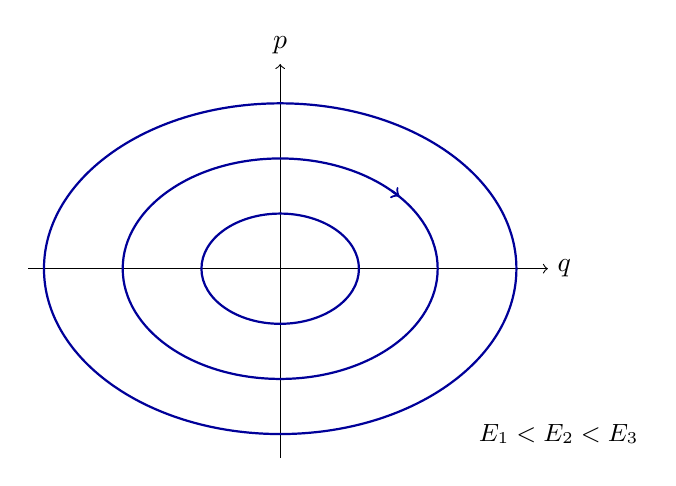
\begin{tikzpicture}[scale=1.0]
 \draw[->] (-3.2,0) -- (3.4,0) node[right] {$q$};
 \draw[->] (0,-2.4) -- (0,2.6) node[above] {$p$};
 \foreach \a/\b in {1/0.7,2/1.4,3/2.1}{
   \draw[blue!60!black,thick] (0,0) ellipse (\a cm and \b cm);
 }
 \draw[blue!60!black,thick,->] (1.414,0.99) -- ++(0.1,-0.07);
 \node[font=\small,right] at (2.4,-2.1) {$E_1<E_2<E_3$};
\end{tikzpicture}
\end{center}

\paragraph{Pendulum.} Take $H=\tfrac12p^2-\cos q$ (setting $m=\ell=g=1$ for the picture). The level curves $p=\pm\sqrt{2(E+\cos q)}$ look like this:
\begin{center}
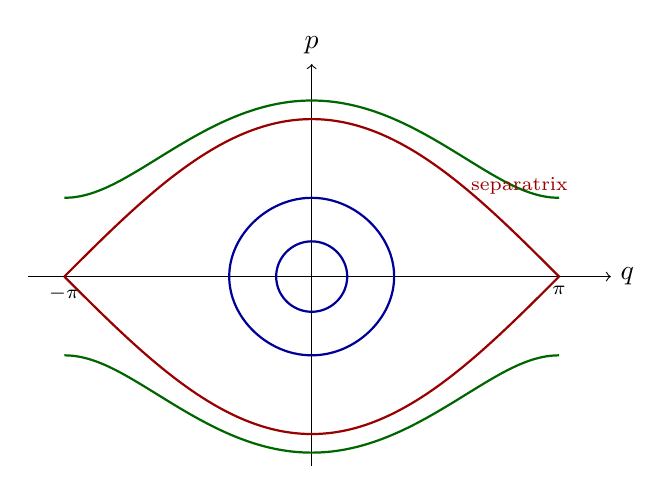
\begin{tikzpicture}[scale=1.0]
 \draw[->] (-3.6,0) -- (3.8,0) node[right] {$q$};
 \draw[->] (0,-2.4) -- (0,2.7) node[above] {$p$};
 \node[below,font=\scriptsize] at (3.14159,0) {$\pi$};
 \node[below,font=\scriptsize] at (-3.14159,0) {$-\pi$};
 % librations
 % closed curves via sin(q/2)=k sin t, p=2k cos t (k=0.2236: E=-0.9; k=0.5: E=-0.5)
 \foreach \k in {0.2236,0.5}{
   \draw[blue!60!black,thick,variable=\t,domain=0:360,samples=90,smooth cycle] plot ({2*asin(\k*sin(\t))*pi/180},{2*\k*cos(\t)});
 }
 % separatrix
 \draw[red!60!black,thick,domain=-3.14159:3.14159,samples=60,smooth] plot (\x,{2*cos(\x/2 r)});
 \draw[red!60!black,thick,domain=-3.14159:3.14159,samples=60,smooth] plot (\x,{-2*cos(\x/2 r)});
 % rotations
 \draw[green!40!black,thick,domain=-3.14159:3.14159,samples=60,smooth] plot (\x,{sqrt(2*(1.5+cos(\x r)))});
 \draw[green!40!black,thick,domain=-3.14159:3.14159,samples=60,smooth] plot (\x,{-sqrt(2*(1.5+cos(\x r)))});
 \node[red!60!black,font=\scriptsize,right] at (1.9,1.15) {separatrix};
 \node[blue!60!black,font=\scriptsize] at (0.0,0.35) {};
\end{tikzpicture}
\end{center}
Closed curves near the origin are \emph{librations} (the pendulum swings, $E<1$), approximately the oscillator ellipses. The \emph{separatrix} $E=1$ (red) has $p=\pm2\cos(q/2)$ and connects the unstable equilibria at $q=\pm\pi$ (the inverted pendulum); a trajectory on it takes infinite time to arrive. Above it ($E>1$, green) the pendulum \emph{rotates} and $q$ increases without bound (with $q$ identified mod $2\pi$, the phase space is really a cylinder).

\paragraph{Liouville's theorem.} The flow \eqref{eq:Hamilton} has velocity field $(\dot q_i,\dot p_i)=(\partial H/\partial p_i,-\partial H/\partial q_i)$ in phase space, whose divergence is
\begin{equation}
 \sum_i\Bigl(\pdiff{\dot q_i}{q_i}+\pdiff{\dot p_i}{p_i}\Bigr)=\sum_i\Bigl(\frac{\partial^2H}{\partial q_i\partial p_i}-\frac{\partial^2H}{\partial p_i\partial q_i}\Bigr)=0 .
\end{equation}
Phase space flows like an incompressible fluid.

\begin{theorem}[Liouville]
The Hamiltonian flow preserves phase-space volume: if a region of phase space is carried along by the flow, its volume $\int\prod_i\dd q_i\,\dd p_i$ does not change.
\end{theorem}

This is what makes statistical mechanics work (a uniform ensemble stays uniform), and it is the classical shadow of unitary time evolution. It has no analogue for the Lagrangian velocity-space $(q,\dot q)$.

%=====================================================================
\section{Poisson brackets}

\subsection{Definition and basic properties}

\begin{definition}
For two functions $A(q,p,t)$ and $B(q,p,t)$ on phase space, the \emph{Poisson bracket} is
\begin{equation}
 \pb AB\equiv\sum_i\Bigl(\pdiff A{q_i}\pdiff B{p_i}-\pdiff A{p_i}\pdiff B{q_i}\Bigr).
\label{eq:PBdef}
\end{equation}
\end{definition}

\begin{pitfall}
\textbf{Sign convention.} We use the convention \eqref{eq:PBdef}, for which $\pb qp=+1$ and $\dot A=\pb AH+\partial_tA$. Some books define the bracket with the opposite overall sign (and then write $\dot A=\pb HA$ or have $\pb pq=1$). Always check which convention a source uses before comparing formulae. The convention here is the one for which the quantization rule reads $\pb AB\to\frac1{i\hbar}[\hat A,\hat B]$ with no extra minus sign.
\end{pitfall}

Directly from the definition one reads off:
\begin{enumerate}[label=(\roman*),nosep]
 \item \textbf{Antisymmetry:} $\pb AB=-\pb BA$; in particular $\pb AA=0$.
 \item \textbf{Bilinearity:} $\pb{\alpha A+\beta B}{C}=\alpha\pb AC+\beta\pb BC$ for constants $\alpha,\beta$.
 \item \textbf{Leibniz rule:} $\pb{AB}{C}=A\pb BC+\pb AC\,B$ (the bracket is a derivation, since it consists of first derivatives).
 \item \textbf{Jacobi identity:} $\pb A{\pb BC}+\pb B{\pb CA}+\pb C{\pb AB}=0$.
\end{enumerate}
Properties (i)--(iii) are immediate. The Jacobi identity can be proved by brute force. Expanded, every term is a product of three factors, exactly one of which is a \emph{second} derivative (of $A$, $B$ or $C$). Collect the terms containing second derivatives of $A$: they come only from $\pb B{\pb CA}$ and $\pb C{\pb AB}$, and they cancel against each other by the symmetry of mixed partial derivatives. The same happens for $B$ and $C$, so the whole sum vanishes. Exercise~\ref{ex:jacobi} asks you to check an instance explicitly.

The fundamental brackets follow from \eqref{eq:PBdef}:
\begin{equation}
 \pb{q_i}{q_j}=0,\qquad \pb{p_i}{p_j}=0,\qquad \pb{q_i}{p_j}=\delta_{ij}.
\label{eq:canonical}
\end{equation}
Combined with the Leibniz rule, these determine the bracket of any two functions. In particular, for any $F(q,p)$,
\begin{equation}
 \pb F{p_i}=\pdiff F{q_i},\qquad \pb F{q_i}=-\pdiff F{p_i}.
\end{equation}

\subsection{Time evolution}

Let $A(q,p,t)$ be any observable. Along a solution of Hamilton's equations,
\begin{align}
 \diff At&=\pdiff At+\sum_i\Bigl(\pdiff A{q_i}\dot q_i+\pdiff A{p_i}\dot p_i\Bigr)
 =\pdiff At+\sum_i\Bigl(\pdiff A{q_i}\pdiff H{p_i}-\pdiff A{p_i}\pdiff H{q_i}\Bigr).
\end{align}

\begin{keyresult}[: Time evolution via Poisson brackets]
\begin{equation}
 \diff At=\pb AH+\pdiff At .
\end{equation}
Hamilton's equations themselves are the special cases $\dot q_i=\pb{q_i}H$ and $\dot p_i=\pb{p_i}H$.
\end{keyresult}

Consequently, a quantity $A$ with no explicit time dependence is conserved if and only if $\pb AH=0$. Taking $A=H$ shows $\dot H=\partial_tH$ again, since $\pb HH=0$. Moreover, if $A$ and $B$ are both conserved, so is $\pb AB$ (``Poisson's theorem''), as the Jacobi identity gives $\diff{}{t}\pb AB=\pb{\pb AH}B+\pb A{\pb BH}$ for time-independent $A,B$, which is $0$ when both brackets with $H$ vanish.

\subsection{Angular momentum}

For a particle in three dimensions, $L_i=\sum_{j,k}\epsilon_{ijk}x_jp_k$, e.g.\ $L_x=yp_z-zp_y$, $L_y=zp_x-xp_z$, $L_z=xp_y-yp_x$. We compute $\pb{L_x}{L_y}$ using bilinearity and the Leibniz rule; only a coordinate with its own momentum gives a nonzero bracket.
\begin{align}
 \pb{L_x}{L_y}&=\pb{yp_z}{zp_x}-\pb{yp_z}{xp_z}-\pb{zp_y}{zp_x}+\pb{zp_y}{xp_z}.
\end{align}
Term by term: $\pb{yp_z}{zp_x}=yp_x\pb{p_z}{z}=-yp_x$; $\pb{yp_z}{xp_z}=0$ (no matching coordinate--momentum pair); $\pb{zp_y}{zp_x}=0$; $\pb{zp_y}{xp_z}=p_yx\pb z{p_z}=xp_y$. Hence $\pb{L_x}{L_y}=xp_y-yp_x=L_z$. By cyclic relabelling,
\begin{equation}
 \pb{L_i}{L_j}=\sum_k\epsilon_{ijk}L_k .
\end{equation}
The same structure holds for the quantum operators: $[\hat L_i,\hat L_j]=i\hbar\epsilon_{ijk}\hat L_k$, which is precisely the rule $[\hat A,\hat B]=i\hbar\widehat{\pb AB}$ applied to these brackets. Also, $\pb{L_i}{x_l}=\sum\epsilon_{ilk}x_k$ and $\pb{L_i}{p_l}=\sum\epsilon_{ilk}p_k$: $\vect L$ generates rotations of vectors (Exercise~\ref{ex:Lbrackets}). A quantity such as $\vect L^2$ or $\vect x\cdot\vect p$ is a rotational scalar, and so has zero bracket with every $L_i$.

%=====================================================================
\section{Canonical transformations}

The coordinates $(q,p)$ are not sacred. A change of phase-space variables $(q,p)\to(Q,P)$ is called \emph{canonical} if the new variables satisfy the same fundamental brackets,
\begin{equation}
 \pb{Q_i}{Q_j}=0,\qquad\pb{P_i}{P_j}=0,\qquad\pb{Q_i}{P_j}=\delta_{ij},
\end{equation}
(brackets evaluated with respect to the old variables). It can be shown that this guarantees that all Poisson brackets are the same whether evaluated in old or new variables, and that Hamilton's equations keep their form $\dot Q=\partial\tilde H/\partial P$, $\dot P=-\partial\tilde H/\partial Q$ (with $\tilde H$ the Hamiltonian re-expressed in the new variables, when the transformation is time independent). For one degree of freedom, $\pb QP=1$ says that the map $(q,p)\mapsto(Q,P)$ has Jacobian determinant $\partial(Q,P)/\partial(q,p)=1$: area preserving.

Since the quantum commutation relations are the images of these brackets, canonical transformations are the classical counterparts of unitary transformations of the quantum theory.

\subsection{The harmonic oscillator in complex variables}
\label{sec:ladder}

This is the central example of the lesson. Take
\begin{equation}
 H=\frac{p^2}{2m}+\frac12m\omega^2q^2 .
\end{equation}
Define the (classical, complex) variable
\begin{equation}
 \boxed{\,a\equiv\sqrt{\frac{m\omega}2}\Bigl(q+\frac{ip}{m\omega}\Bigr),\qquad a^*=\sqrt{\frac{m\omega}2}\Bigl(q-\frac{ip}{m\omega}\Bigr).\,}
\label{eq:adef}
\end{equation}
\emph{Normalization:} with this choice $a$ has dimensions of $\sqrt{\text{action}}$ (you can check: $\sqrt{m\omega}\,q$ has dimensions $\sqrt{\text{mass}\cdot\text{length}^2/\text{time}}$). The quantum ladder operator is $\hat a=\hat a_{\rm cl}/\sqrt\hbar$, as we will see.

It is helpful to note that $a=(Q+iP)/\sqrt2$ with the rescaled variables $Q=\sqrt{m\omega}\,q$, $P=p/\sqrt{m\omega}$. The rescaling is canonical: $\pb QP=\pb qp=1$. And $H=\tfrac\omega2(Q^2+P^2)$.

\paragraph{Hamiltonian.} Compute
\begin{equation}
 a^*a=\frac{m\omega}2\Bigl(q^2+\frac{p^2}{m^2\omega^2}\Bigr)=\frac{m\omega q^2}2+\frac{p^2}{2m\omega},
\end{equation}
so
\begin{equation}
 H=\omega\,a^*a .
\end{equation}

\paragraph{Bracket.} Using bilinearity and $\pb qq=\pb pp=0$,
\begin{align}
 \pb a{a^*}&=\frac{m\omega}2\Bigl\{q+\frac{ip}{m\omega},\,q-\frac{ip}{m\omega}\Bigr\}
 =\frac{m\omega}2\Bigl(-\frac i{m\omega}\pb qp+\frac i{m\omega}\pb pq\Bigr)\nonumber\\
 &=\frac{m\omega}{2}\cdot\frac{-2i}{m\omega}=-i .
\end{align}
So
\begin{equation}
 \pb a{a^*}=-i,\qquad \pb aa=\pb{a^*}{a^*}=0 .
\end{equation}

\paragraph{Time evolution.} Since $a$ has no explicit time dependence,
\begin{equation}
 \dot a=\pb aH=\omega\pb a{a^*a}=\omega\pb a{a^*}a=-i\omega\,a ,
\end{equation}
(using the Leibniz rule and $\pb aa=0$). Hence
\begin{equation}
 a(t)=a(0)\,e^{-i\omega t},\qquad a^*(t)=a^*(0)e^{+i\omega t}.
\end{equation}
The motion in the complex $a$-plane is a uniform rotation at angular frequency $\omega$; $|a|^2=H/\omega$ is constant. Recovering the real variable,
\begin{equation}
 q=\frac{a+a^*}{\sqrt{2m\omega}},\qquad p=-i\sqrt{\frac{m\omega}2}\,(a-a^*),
\label{eq:qpfroma}
\end{equation}
so $q(t)=\sqrt{2/m\omega}\,|a|\cos(\omega t-\delta)$ for $a(0)=|a|e^{i\delta}$ (check: $q_{\max}=\sqrt{2|a|^2/m\omega}=\sqrt{2E/m\omega^2}$ \checkmark).

\subsection{Link to the quantum ladder operators}

Apply the rule $\pb AB\to\frac1{i\hbar}[\hat A,\hat B]$, i.e.\ $[\hat A,\hat B]=i\hbar\,\widehat{\pb AB}$, to the bracket $\pb a{a^*}=-i$:
\begin{equation}
 [\hat a_{\rm cl},\hat a_{\rm cl}^\dagger]=i\hbar\cdot(-i)=\hbar .
\end{equation}
Defining $\hat a\equiv\hat a_{\rm cl}/\sqrt\hbar$ we obtain the famous
\begin{equation}
 \boxed{[\hat a,\hat a^\dagger]=1},\qquad \hat q=\sqrt{\frac{\hbar}{2m\omega}}\,(\hat a+\hat a^\dagger),\qquad \hat p=-i\sqrt{\frac{\hbar m\omega}2}\,(\hat a-\hat a^\dagger),
\end{equation}
and $\hat H=\hbar\omega\,\hat a^\dagger\hat a$ (plus a constant $\tfrac12\hbar\omega$ from an ordering choice, see below). The Heisenberg equation then gives $\dot{\hat a}=\frac1{i\hbar}[\hat a,\hat H]=\frac1{i\hbar}\hbar\omega\hat a=-i\omega\hat a$, matching $\dot a=-i\omega a$. The entire algebraic structure of the quantum oscillator is already present in $\pb a{a^*}=-i$.

\begin{qftbridge}
This is the key step toward the QFT strategy of L\&B. A free field is an infinite collection of decoupled oscillators, one per momentum mode $\vect k$, each with its own $a_{\vect k},a_{\vect k}^\dagger$. The occupation-number picture (second quantization) of L\&B's early chapters and the mode expansion of the scalar field in ch.~11 are the sum over modes of exactly what you just derived. The ``$a_{\vect k}$'' of the field theory is the classical amplitude $a$ of a normal mode, with the same time dependence $e^{-i\omega_{\vect k}t}$.
\end{qftbridge}

%=====================================================================
\section{Dirac's quantization rule}
\label{sec:dirac}

\begin{keyresult}[: Canonical quantization]
Promote phase-space functions to operators and replace Poisson brackets by commutators:
\begin{equation}
 \pb AB\ \longrightarrow\ \frac1{i\hbar}\comm{\hat A}{\hat B},\qquad\text{in particular}\quad \comm{\hat q_i}{\hat p_j}=i\hbar\,\delta_{ij},\quad\comm{\hat q_i}{\hat q_j}=\comm{\hat p_i}{\hat p_j}=0 .
\end{equation}
\end{keyresult}

\paragraph{Heisenberg equation mirrors Hamilton.} In the Heisenberg picture, $\hat A_H(t)=e^{i\hat Ht/\hbar}\hat Ae^{-i\hat Ht/\hbar}$, and differentiating gives
\begin{equation}
 \diff{\hat A_H}t=\frac i\hbar\comm{\hat H}{\hat A_H}+\Bigl(\pdiff{\hat A}t\Bigr)_H=\frac1{i\hbar}\comm{\hat A_H}{\hat H}+\Bigl(\pdiff{\hat A}t\Bigr)_H .
\end{equation}
Compare with $\dot A=\pb AH+\partial_tA$: the Heisenberg equation is the Poisson-bracket equation with $\pb{\ }{\ }\to\frac1{i\hbar}[\ ,\ ]$. The properties of the bracket (antisymmetry, bilinearity, Leibniz, Jacobi) are all properties that the commutator also has, which is why the replacement is consistent. The classical limit $\hbar\to0$ is the statement that commutators become $i\hbar$ times Poisson brackets.

\paragraph{Ordering ambiguities.} Classically $qp=pq$, but $\hat q\hat p\neq\hat p\hat q$. So a function such as $qp$ or $p^2q^2$ does not determine a unique operator: $\hat q\hat p$, $\hat p\hat q$, and $\tfrac12(\hat q\hat p+\hat p\hat q)$ all reduce to $qp$ as $\hbar\to0$. The Hamiltonian of the oscillator shows it: $\omega a^*a$ could be quantized as $\hbar\omega\,\hat a^\dagger\hat a$ or as $\tfrac12\hbar\omega(\hat a^\dagger\hat a+\hat a\hat a^\dagger)=\hbar\omega(\hat a^\dagger\hat a+\tfrac12)$, differing by the zero-point energy. In field theory this constant, summed over infinitely many modes, becomes a divergent vacuum energy, handled in L\&B by normal ordering. Note also that the correspondence cannot hold for \emph{all} functions at once (the Groenewold--van~Hove no-go theorem); it works for the basic variables and low-order polynomials.

%=====================================================================
\section{Hamiltonian field theory}
\label{sec:fieldHam}

From now on $\hbar=c=1$ and the metric is $(+,-,-,-)$.

\subsection{From many particles to a continuum}

Recall from Lesson 1 that a field theory has Lagrangian $L=\int\dd^3x\,\Lag(\phi,\partial_\mu\phi)$. The field value $\phi(\vect x,t)$ at each point $\vect x$ plays the role of a coordinate $q_i$ (the index $i$ has become the continuous label $\vect x$). The canonical momentum conjugate to $\phi(\vect x)$ is defined by the same recipe, applied to the \emph{density}:
\begin{equation}
 \pi(\vect x,t)\equiv\pdiff{\Lag}{\dot\phi(\vect x,t)},\qquad \Ham\equiv\pi\dot\phi-\Lag,\qquad H=\int\dd^3x\,\Ham .
\end{equation}
(For several fields, $\sum_a\pi_a\dot\phi_a$.) To see why this is right, discretize space into cells of volume $\Delta V$ labelled by $i$: then $L=\sum_i\Delta V\,\Lag_i$, the momentum conjugate to $\phi_i$ is $\partial L/\partial\dot\phi_i=\Delta V\,\pi_i$, and $H=\sum_i p_i\dot\phi_i-L=\sum_i\Delta V(\pi_i\dot\phi_i-\Lag_i)$, which becomes $\int\Ham\,\dd^3x$.

\begin{pitfall}
$\pi$ is a momentum \emph{density}: it is the momentum per unit volume, $p_i\to\Delta V\,\pi(\vect x_i)$. This is why the continuum bracket involves $\delta^3(\vect x-\vect y)$ rather than a Kronecker delta: $\delta_{ij}/\Delta V\to\delta^3(\vect x-\vect y)$.
\end{pitfall}

\subsection{Example 1: the vibrating string}

For a string with linear mass density $\rho$, tension $T$ and displacement $\phi(x,t)$, Lesson~1 gave $\Lag=\tfrac12\rho\dot\phi^2-\tfrac12T\phi'^2$ (a prime is $\partial_x$). Then
\begin{equation}
 \pi=\pdiff\Lag{\dot\phi}=\rho\dot\phi,\qquad \Ham=\pi\dot\phi-\Lag=\frac{\pi^2}{2\rho}+\frac12T\phi'^2 .
\end{equation}
Kinetic plus potential energy density, as expected for a natural system. Hamilton's equations (derived properly below) give $\dot\phi=\pi/\rho$ and $\dot\pi=T\phi''$, so $\ddot\phi=(T/\rho)\phi''$: the wave equation with speed $\sqrt{T/\rho}$.

\subsection{Example 2: the Klein--Gordon field}

For the real scalar field, with signature $(+,-,-,-)$,
\begin{equation}
 \Lag=\tfrac12\partial_\mu\phi\,\partial^\mu\phi-\tfrac12m^2\phi^2=\tfrac12\dot\phi^2-\tfrac12(\nabla\phi)^2-\tfrac12m^2\phi^2 .
\end{equation}
Therefore
\begin{equation}
 \pi=\pdiff\Lag{\dot\phi}=\dot\phi,
\end{equation}
and
\begin{equation}
 \Ham=\pi\dot\phi-\Lag=\dot\phi^2-\tfrac12\dot\phi^2+\tfrac12(\nabla\phi)^2+\tfrac12m^2\phi^2
 \ \Longrightarrow\ \boxed{\Ham=\tfrac12\pi^2+\tfrac12(\nabla\phi)^2+\tfrac12m^2\phi^2 .}
\end{equation}
Again note that $\Ham$ is written in terms of $\pi$, not $\dot\phi$. Each term is non-negative, so the energy is bounded below.

\subsection{Field Poisson brackets and Hamilton's equations}

To define brackets we need derivatives with respect to a function. For a functional $F[\phi,\pi]$, the \emph{functional derivative} $\delta F/\delta\phi(\vect x)$ is defined by the first-order change
\begin{equation}
 \delta F=\int\dd^3x\,\fdiff F{\phi(\vect x)}\,\delta\phi(\vect x)+\int\dd^3x\,\fdiff F{\pi(\vect x)}\,\delta\pi(\vect x).
\end{equation}
In particular $\delta\phi(\vect x)/\delta\phi(\vect y)=\delta^3(\vect x-\vect y)$. The field Poisson bracket is the obvious continuum limit of \eqref{eq:PBdef}, with the sum over $i$ replaced by an integral over $\vect z$:
\begin{equation}
 \pb FG\equiv\int\dd^3z\Bigl(\fdiff F{\phi(\vect z)}\fdiff G{\pi(\vect z)}-\fdiff F{\pi(\vect z)}\fdiff G{\phi(\vect z)}\Bigr),
\end{equation}
with all fields evaluated at the same time. Taking $F=\phi(\vect x)$ and $G=\pi(\vect y)$,
\begin{equation}
 \boxed{\pb{\phi(\vect x,t)}{\pi(\vect y,t)}=\delta^3(\vect x-\vect y),\qquad\pb{\phi(\vect x,t)}{\phi(\vect y,t)}=\pb{\pi(\vect x,t)}{\pi(\vect y,t)}=0 .}
\end{equation}
Equal times are essential. Time evolution is again generated by $H$: for $F$ without explicit time dependence, $\dot F=\pb FH$. Hence $\dot\phi(\vect x)=\pb{\phi(\vect x)}H=\delta H/\delta\pi(\vect x)$ and $\dot\pi(\vect x)=\pb{\pi(\vect x)}{H}=-\delta H/\delta\phi(\vect x)$.

\paragraph{Klein--Gordon equation from Hamilton.} Take $H=\int\dd^3x\,[\tfrac12\pi^2+\tfrac12(\nabla\phi)^2+\tfrac12m^2\phi^2]$. Varying $\pi$: $\delta H=\int\pi\,\delta\pi$, so $\delta H/\delta\pi=\pi$. Varying $\phi$, and integrating by parts (assuming $\delta\phi$ vanishes at infinity):
\begin{equation}
 \delta H=\int\dd^3x\,[\nabla\phi\cdot\nabla\delta\phi+m^2\phi\,\delta\phi]=\int\dd^3x\,[-\nabla^2\phi+m^2\phi]\,\delta\phi,
\end{equation}
so $\delta H/\delta\phi=-\nabla^2\phi+m^2\phi$. Hamilton's equations are therefore
\begin{equation}
 \dot\phi=\pi,\qquad\dot\pi=\nabla^2\phi-m^2\phi .
\end{equation}
Eliminating $\pi$:
\begin{equation}
 \ddot\phi-\nabla^2\phi+m^2\phi=0\quad\Longleftrightarrow\quad(\partial_\mu\partial^\mu+m^2)\phi=0,
\end{equation}
the Klein--Gordon equation, as found from the Euler--Lagrange equation in Lesson~1.

\begin{qftbridge}
\textbf{Canonical quantization of the scalar field (L\&B ch.~11).} Promoting $\phi,\pi$ to operators with the rule $\pb{\ }{\ }\to\frac1{i}[\ ,\ ]$ (with $\hbar=1$) turns the field brackets into the equal-time commutation relations
\[
 \comm{\hat\phi(\vect x)}{\hat\pi(\vect y)}=i\,\delta^3(\vect x-\vect y),\qquad\comm{\hat\phi(\vect x)}{\hat\phi(\vect y)}=\comm{\hat\pi(\vect x)}{\hat\pi(\vect y)}=0 .
\]
Expanding the classical solution in Fourier modes, each mode is a harmonic oscillator of frequency $\omega_{\vect k}=\sqrt{\vect k^2+m^2}$ with its own complex amplitude $a_{\vect k}$ obeying $\dot a_{\vect k}=-i\omega_{\vect k}a_{\vect k}$, precisely the solution of Section~\ref{sec:ladder}. Quantizing those amplitudes gives $[\hat a_{\vect k},\hat a_{\vect k'}^\dagger]\propto\delta^3(\vect k-\vect k')$, and the Fock space of particles follows. Everything in this lesson is the groundwork for that derivation.
\end{qftbridge}

\begin{pitfall}
Because $\pi$ is a density, $\pb{\phi(\vect x)}{\pi(\vect y)}$ is a delta \emph{function}; products such as $\hat\phi(\vect x)^2$ then carry infinite zero-point contributions. That is the origin of the divergences that normal ordering and renormalization deal with in L\&B.
\end{pitfall}

%=====================================================================
\section{Summary: what to know cold}

\begin{itemize}[nosep]
 \item $p_i=\partial L/\partial\dot q_i$; for a charged particle $\vect p=m\dot{\vect x}+q\vect A$. Cyclic coordinate $\Rightarrow$ conserved $p_i$.
 \item $H(q,p,t)=\sum p_i\dot q_i-L$, written in terms of $p$. $\dot q_i=\partial H/\partial p_i$, $\dot p_i=-\partial H/\partial q_i$, $\partial_tH=-\partial_tL$; $\dot H=\partial_tH$.
 \item $H=T+V$ only for natural systems (quadratic $T$ with time-independent coefficients, $V(q)$). $H$ conserved $\neq$ $H$ equals energy.
 \item Phase-space trajectories are level sets of $H$ (for $N=1$); Liouville: the flow preserves volume.
 \item $\pb AB=\sum(\partial_{q}A\,\partial_pB-\partial_pA\,\partial_qB)$; antisymmetric, bilinear, Leibniz, Jacobi; $\pb{q_i}{p_j}=\delta_{ij}$; $\dot A=\pb AH+\partial_tA$.
 \item $\pb{L_i}{L_j}=\epsilon_{ijk}L_k$.
 \item Canonical transformations preserve $\pb{q}{p}=1$. Oscillator: $a=\sqrt{m\omega/2}\,(q+ip/m\omega)$, $H=\omega a^*a$, $\pb a{a^*}=-i$, $a(t)=a(0)e^{-i\omega t}$.
 \item Quantization: $\pb AB\to\frac1{i\hbar}[\hat A,\hat B]$; Heisenberg $\dot{\hat A}=\frac1{i\hbar}[\hat A,\hat H]$; $[\hat a,\hat a^\dagger]=1$ for $\hat a=a/\sqrt\hbar$; ordering ambiguities.
 \item Fields: $\pi=\partial\Lag/\partial\dot\phi$, $\Ham=\pi\dot\phi-\Lag$; KG: $\Ham=\tfrac12\pi^2+\tfrac12(\nabla\phi)^2+\tfrac12m^2\phi^2$; $\pb{\phi(\vect x)}{\pi(\vect y)}=\delta^3(\vect x-\vect y)$; $\dot\phi=\delta H/\delta\pi$, $\dot\pi=-\delta H/\delta\phi$.
\end{itemize}

\paragraph{Suggested further reading.}
\begin{itemize}[nosep]
 \item L.~Susskind and G.~Hrabovsky, \emph{The Theoretical Minimum: What You Need to Know to Start Doing Physics} (classical mechanics), Lectures~8--10: Hamiltonian mechanics, the phase-space fluid and Liouville's theorem, and Poisson brackets.
 \item H.~Goldstein, C.~Poole and J.~Safko, \emph{Classical Mechanics}, the chapters on the Hamilton equations of motion and on canonical transformations and Poisson brackets (chs.~8--9 of the 3rd edition).
 \item D.~Tong, \emph{Classical Dynamics}, Cambridge lecture notes (freely available on his website), the chapter on Hamiltonian formalism.
\end{itemize}

%=====================================================================
\section{Exercises}

\begin{exercise}[central potential in polar coordinates]\label{ex:central}
A particle of mass $m$ moves in a plane under a central potential $V(r)$. Write the Lagrangian in polar coordinates $(r,\theta)$, find $p_r$ and $p_\theta$, and construct the Hamiltonian. Write Hamilton's equations and identify the conserved quantity. Interpret the term $p_\theta^2/2mr^2$.
\end{exercise}

\begin{exercise}[charged particle]\label{ex:charged}
(a) Starting from \eqref{eq:Lcharged}, show that the Euler--Lagrange equations give the Lorentz force law $m\ddot{\vect x}=q(\vect E+\dot{\vect x}\times\vect B)$ with $\vect E=-\nabla\varphi-\partial_t\vect A$, $\vect B=\nabla\times\vect A$. (b) Show that the Hamiltonian is $H=(\vect p-q\vect A)^2/2m+q\varphi$. (c) Show $\dot{\vect x}=(\vect p-q\vect A)/m$ follows from Hamilton's equations.
\end{exercise}

\begin{exercise}[the relativistic particle]\label{ex:relativistic}
With $c=1$, the Lagrangian of a free relativistic particle is $L=-m\sqrt{1-\dot{\vect x}^2}$. Find $\vect p$, then show $H=\sqrt{\vect p^2+m^2}$. Expand for small $|\vect p|$ and comment.
\end{exercise}

\begin{exercise}[Jacobi identity]\label{ex:jacobi}
For one degree of freedom take $A=q$, $B=p^2$, $C=q^2p$. Compute $\pb A{\pb BC}+\pb B{\pb CA}+\pb C{\pb AB}$ and verify it vanishes.
\end{exercise}

\begin{exercise}[angular momentum brackets]\label{ex:Lbrackets}
Let $\vect L=\vect x\times\vect p$ for a particle in 3D. (a) Compute $\pb{L_z}{x}$, $\pb{L_z}y$, $\pb{L_z}z$ and $\pb{L_z}{p_x}$. (b) Compute $\pb{L_z}{r^2}$ where $r^2=x^2+y^2+z^2$ and $\pb{L_z}{\vect p^2}$. Conclude that $L_z$ is conserved for $H=\vect p^2/2m+V(r)$. (c) Derive $\pb{L_y}{L_z}=L_x$.
\end{exercise}

\begin{exercise}[canonical transformations]\label{ex:canonical}
Decide which of these maps $(q,p)\mapsto(Q,P)$ are canonical: (a) $Q=q\cos\alpha+p\sin\alpha$, $P=-q\sin\alpha+p\cos\alpha$; (b) $Q=q^2$, $P=p/(2q)$ (for $q>0$); (c) $Q=2q$, $P=2p$; (d) $Q=p$, $P=-q$. For (d), take $H=p^2/2m+V(q)$ and write $H$ in the new variables, commenting on the role reversal of coordinate and momentum.
\end{exercise}

\begin{exercise}[damped oscillator]\label{ex:damped}
Consider $L=e^{\gamma t}\bigl(\tfrac12m\dot q^2-\tfrac12kq^2\bigr)$. (a) Show that the Euler--Lagrange equation is the damped oscillator equation $m(\ddot q+\gamma\dot q)+kq=0$. (b) Find $p$ and $H(q,p,t)$. (c) Write down Hamilton's equations and check $\partial_tH=-\partial_tL$. (d) Show that $H=e^{\gamma t}E$ with $E=\tfrac12m\dot q^2+\tfrac12kq^2$ the mechanical energy, and that $H$ is not conserved, but also that $H\ne E$.
\end{exercise}

\begin{exercise}[ladder variables]\label{ex:ladder}
For $H=p^2/2m+\tfrac12m\omega^2q^2$ and $a=\sqrt{m\omega/2}\,(q+ip/m\omega)$: (a) show $\pb a{a^*}=-i$ and $H=\omega a^*a$; (b) derive $\dot a=-i\omega a$ both from $\dot a=\pb aH$ and directly from Hamilton's equations in $(q,p)$; (c) express $q(t)$ in terms of $a(0)$; (d) find the quantum commutator $[\hat a,\hat a^\dagger]$ for $\hat a=a/\sqrt\hbar$ via Dirac's rule.
\end{exercise}

\begin{exercise}[a self-interacting scalar field]\label{ex:phi4}
Let $\Lag=\tfrac12\partial_\mu\phi\,\partial^\mu\phi-\tfrac14\lambda\phi^4$ (signature $(+,-,-,-)$, $\lambda>0$). (a) Find $\pi$ and $\Ham$. (b) Derive Hamilton's equations for $\phi$ and $\pi$ and combine them into a second-order field equation. (c) Confirm that it agrees with the Euler--Lagrange equation.
\end{exercise}

\begin{exercise}[the complex scalar field]\label{ex:complex}
Let $\Lag=\partial_\mu\psi^*\partial^\mu\psi-m^2\psi^*\psi$, treating $\psi$ and $\psi^*$ as independent fields. (a) Find the two conjugate momenta $\pi_\psi$, $\pi_{\psi^*}$ and the Hamiltonian density. (b) Write the nonzero equal-time brackets. (c) Show that Hamilton's equations reproduce $(\partial^2+m^2)\psi=0$.
\end{exercise}

%=====================================================================
\section{Solutions}

\begin{solution}{ex:central}
In polar coordinates $\dot x^2+\dot y^2=\dot r^2+r^2\dot\theta^2$, so $L=\tfrac12m(\dot r^2+r^2\dot\theta^2)-V(r)$. Then $p_r=m\dot r$ and $p_\theta=mr^2\dot\theta$, so $\dot r=p_r/m$, $\dot\theta=p_\theta/mr^2$. Hence
\[
 H=p_r\dot r+p_\theta\dot\theta-L=\frac{p_r^2}{m}+\frac{p_\theta^2}{mr^2}-\frac{p_r^2}{2m}-\frac{p_\theta^2}{2mr^2}+V
 =\frac{p_r^2}{2m}+\frac{p_\theta^2}{2mr^2}+V(r).
\]
Hamilton's equations: $\dot r=p_r/m$, $\dot\theta=p_\theta/mr^2$, $\dot p_r=-\partial H/\partial r=p_\theta^2/(mr^3)-V'(r)$, $\dot p_\theta=-\partial H/\partial\theta=0$. So $p_\theta=\ell$ is conserved (the angular momentum; $\theta$ is cyclic). Substituting $\ell$ turns the radial motion into a one-dimensional problem with effective potential $V_{\rm eff}=V+\ell^2/2mr^2$: the second term is the centrifugal barrier. Also $\dot p_r=m\ddot r$ gives $m\ddot r=\ell^2/mr^3-V'$, the familiar radial equation.
\end{solution}

\begin{solution}{ex:charged}
(a) $\partial L/\partial\dot x_i=m\dot x_i+qA_i$, so $\diff{}{t}(m\dot x_i+qA_i)=m\ddot x_i+q(\partial_tA_i+\dot x_j\partial_jA_i)$. And $\partial L/\partial x_i=-q\partial_i\varphi+q\dot x_j\partial_iA_j$. Equating,
\[
 m\ddot x_i=-q\partial_i\varphi-q\partial_tA_i+q\dot x_j(\partial_iA_j-\partial_jA_i)=qE_i+q\,[\dot{\vect x}\times(\nabla\times\vect A)]_i,
\]
using the identity $[\vect v\times(\nabla\times\vect A)]_i=v_j\partial_iA_j-v_j\partial_jA_i$. This is the Lorentz force.

(b) $\vect p=m\dot{\vect x}+q\vect A$ gives $\dot{\vect x}=(\vect p-q\vect A)/m$. Then
\[
 H=\vect p\cdot\dot{\vect x}-L=\vect p\cdot\dot{\vect x}-\tfrac12m\dot{\vect x}^2+q\varphi-q\dot{\vect x}\cdot\vect A=(\vect p-q\vect A)\cdot\dot{\vect x}-\tfrac12m\dot{\vect x}^2+q\varphi=\tfrac12m\dot{\vect x}^2+q\varphi,
\]
and substituting $\dot{\vect x}=(\vect p-q\vect A)/m$: $H=(\vect p-q\vect A)^2/2m+q\varphi$.

(c) $\dot x_i=\partial H/\partial p_i=(p_i-qA_i)/m$. (For completeness, $\dot p_i=-\partial H/\partial x_i=\tfrac qm(p_j-qA_j)\partial_iA_j-q\partial_i\varphi$, which reproduces part (a) after substituting $p_j-qA_j=m\dot x_j$ and $\dot p_i=m\ddot x_i+q\dot A_i$.)
\end{solution}

\begin{solution}{ex:relativistic}
$\vect p=\partial L/\partial\dot{\vect x}=m\dot{\vect x}/\sqrt{1-\dot{\vect x}^2}\equiv m\gamma\dot{\vect x}$. Then $\vect p^2=m^2\gamma^2v^2$, and $\gamma^2=1/(1-v^2)$ implies $\gamma^2v^2=\gamma^2-1$, so $\vect p^2+m^2=m^2\gamma^2$. Now
\[
 H=\vect p\cdot\dot{\vect x}-L=m\gamma v^2+m/\gamma=m\gamma\,(v^2+1-v^2)=m\gamma=\sqrt{\vect p^2+m^2}.
\]
For small $p$: $H\approx m+\vect p^2/2m-\vect p^4/8m^3$: rest energy, the Newtonian kinetic energy, and the first relativistic correction. This $H$, with $\vect p\to-i\nabla$, is the origin of the square root in the single-particle relativistic energy $E_{\vect p}=\sqrt{\vect p^2+m^2}=\omega_{\vect k}$ that appears in every mode of the Klein--Gordon field. Note $H\neq T+V$ here: the Lagrangian is not of the form $T-V$.
\end{solution}

\begin{solution}{ex:jacobi}
Use $\pb AB=\partial_qA\,\partial_pB-\partial_pA\,\partial_qB$.
First, $\pb BC=\pb{p^2}{q^2p}=0-(2p)(2qp)=-4qp^2$, so $\pb A{\pb BC}=\pb q{-4qp^2}=1\cdot(-8qp)=-8qp$.
Second, $\pb CA=\pb{q^2p}{q}=0-(q^2)(1)=-q^2$, so $\pb B{\pb CA}=\pb{p^2}{-q^2}=0-(2p)(-2q)=4qp$.
Third, $\pb AB=\pb q{p^2}=2p$, so $\pb C{\pb AB}=\pb{q^2p}{2p}=(2qp)(2)-0=4qp$.
Sum: $-8qp+4qp+4qp=0$. \checkmark
\end{solution}

\begin{solution}{ex:Lbrackets}
(a) $L_z=xp_y-yp_x$. $\pb{L_z}x=\pb{xp_y}{x}-\pb{yp_x}{x}=0-y\pb{p_x}{x}=y$. $\pb{L_z}y=x\pb{p_y}{y}=-x$. $\pb{L_z}z=0$. $\pb{L_z}{p_x}=\pb{xp_y}{p_x}=p_y\pb x{p_x}=p_y$ (and the $yp_x$ term gives zero). So $L_z$ rotates $(x,y)\to(y,-x)$ and $(p_x,p_y)\to(p_y,-p_x)$ as a generator of rotations about $z$, in agreement with $\pb{L_i}{x_l}=\epsilon_{ilk}x_k$ ($i=z,l=x$: $\epsilon_{zxy}y=y$ \checkmark).

(b) By the chain rule for brackets (Leibniz), $\pb{L_z}{r^2}=2x\pb{L_z}x+2y\pb{L_z}y+2z\pb{L_z}z=2xy-2yx+0=0$. Similarly $\pb{L_z}{\vect p^2}=2p_x\pb{L_z}{p_x}+2p_y\pb{L_z}{p_y}$, and $\pb{L_z}{p_y}=\pb{-yp_x}{p_y}=-p_x\pb y{p_y}=-p_x$, giving $2p_xp_y-2p_yp_x=0$. Hence for $H=\vect p^2/2m+V(r)$, $\pb{L_z}H=\frac1{2m}\pb{L_z}{\vect p^2}+V'(r)\pb{L_z}{r}=0$, so $\dot L_z=0$; same for the other components by symmetry.

(c) $L_y=zp_x-xp_z$, $L_z=xp_y-yp_x$. Expand $\pb{L_y}{L_z}=\pb{zp_x}{xp_y}-\pb{zp_x}{yp_x}-\pb{xp_z}{xp_y}+\pb{xp_z}{yp_x}$ and keep only matching coordinate--momentum pairs. First term: only $p_x$ with $x$, giving $zp_y\pb{p_x}{x}=-zp_y$. Second: $z,p_x$ against $y,p_x$: no pair, $0$. Third: $x,p_z$ against $x,p_y$: no pair, $0$. Fourth: only $x$ with $p_x$, giving $p_z\,y\,\pb x{p_x}=yp_z$. Hence $\pb{L_y}{L_z}=yp_z-zp_y=L_x$. \checkmark
\end{solution}

\begin{solution}{ex:canonical}
Compute $\pb QP=\partial_qQ\,\partial_pP-\partial_pQ\,\partial_qP$ (the only nontrivial bracket for one degree of freedom).

(a) $\pb QP=\cos\alpha\cos\alpha-\sin\alpha(-\sin\alpha)=1$. Canonical (a rotation in phase space, area preserving).

(b) $\pb QP=(2q)\cdot\frac1{2q}-0=1$. Canonical.

(c) $\pb QP=2\cdot2=4\ne1$. Not canonical (it magnifies areas by $4$). Rescaling $Q=\lambda q$ requires $P=p/\lambda$.

(d) $\pb QP=\pb p{-q}=-\pb pq=+1$. Canonical. In new variables $q=-P$, $p=Q$, so $H=Q^2/2m+V(-P)$: the roles of coordinate and momentum are exchanged (up to a sign). This is the classical statement of the position--momentum symmetry underlying the Fourier transform between wavefunctions $\psi(q)$ and $\tilde\psi(p)$; phase space has no canonical distinction between ``coordinates'' and ``momenta''.
\end{solution}

\begin{solution}{ex:damped}
(a) $\partial L/\partial\dot q=e^{\gamma t}m\dot q$, $\partial L/\partial q=-e^{\gamma t}kq$. EL: $\diff{}{t}(e^{\gamma t}m\dot q)=e^{\gamma t}m(\ddot q+\gamma\dot q)=-e^{\gamma t}kq$, i.e.\ $m(\ddot q+\gamma\dot q)+kq=0$.

(b) $p=e^{\gamma t}m\dot q$, so $\dot q=e^{-\gamma t}p/m$. Then $H=p\dot q-L=e^{-\gamma t}p^2/m-e^{\gamma t}\tfrac12m\dot q^2+\tfrac12e^{\gamma t}kq^2=\dfrac{e^{-\gamma t}p^2}{2m}+\tfrac12e^{\gamma t}kq^2$.

(c) $\dot q=\partial H/\partial p=e^{-\gamma t}p/m$; $\dot p=-\partial H/\partial q=-e^{\gamma t}kq$. Also $\partial_tH=-\tfrac\gamma2\frac{e^{-\gamma t}p^2}{m}+\tfrac\gamma2e^{\gamma t}kq^2$, and $-\partial_tL=-\gamma e^{\gamma t}(\tfrac12m\dot q^2-\tfrac12kq^2)$; with $p=e^{\gamma t}m\dot q$ the first is $-\tfrac\gamma2e^{\gamma t}m\dot q^2+\tfrac\gamma2e^{\gamma t}kq^2$, equal to the second. \checkmark

(d) $e^{-\gamma t}p^2/2m=e^{\gamma t}\tfrac12m\dot q^2$, so $H=e^{\gamma t}(\tfrac12m\dot q^2+\tfrac12kq^2)=e^{\gamma t}E$. $H$ is not conserved because $\partial_tH\neq0$. The actual mechanical energy $E$ decreases: $\dot E=m\dot q\ddot q+kq\dot q=\dot q(-m\gamma\dot q)=-\gamma m\dot q^2$. Indeed $\dot H=\gamma H+e^{\gamma t}\dot E=e^{\gamma t}(\gamma E-\gamma m\dot q^2)=\tfrac{\gamma}2e^{\gamma t}(kq^2-m\dot q^2)$, consistent with $\partial_tH$. So $H$, which the formalism keeps in a perfectly well-defined way, is neither constant nor the energy; the dissipation is encoded in the explicit time dependence of $L$ (a trick that works for one-dimensional linear damping).
\end{solution}

\begin{solution}{ex:ladder}
(a) Done in the text: $\pb a{a^*}=\frac{m\omega}2\bigl(-\frac i{m\omega}\pb qp+\frac i{m\omega}\pb pq\bigr)=-i$ and $a^*a=\frac{m\omega}2q^2+\frac{p^2}{2m\omega}$, so $H=\omega a^*a$. Explicitly in the bracket the cross terms are $\pb q{-\frac{ip}{m\omega}}=-\frac i{m\omega}$ and $\pb{\frac{ip}{m\omega}}{q}=-\frac i{m\omega}$, total $-\frac{2i}{m\omega}$, times $\frac{m\omega}2$ gives $-i$.

(b) $\dot a=\pb aH=\omega\pb a{a^*a}=\omega(\pb a{a^*}a+a^*\pb aa)=-i\omega a$. Directly: $\dot q=p/m$, $\dot p=-m\omega^2q$, so $\dot a=\sqrt{\tfrac{m\omega}2}\bigl(\tfrac pm-\tfrac{i}{m\omega}m\omega^2q\bigr)=\sqrt{\tfrac{m\omega}2}\bigl(\tfrac pm-i\omega q\bigr)=-i\omega\sqrt{\tfrac{m\omega}2}\bigl(q+\tfrac{ip}{m\omega}\bigr)=-i\omega a$ \checkmark. Solution $a(t)=a(0)e^{-i\omega t}$.

(c) $q=(a+a^*)/\sqrt{2m\omega}$, so with $a(0)=|a|e^{i\delta}$: $q(t)=\dfrac{2|a|}{\sqrt{2m\omega}}\cos(\omega t-\delta)=\sqrt{\dfrac2{m\omega}}\,|a|\cos(\omega t-\delta)$. Equivalently $q(t)=\mathrm{Re}\bigl[\sqrt{2/m\omega}\,a(0)e^{-i\omega t}\bigr]$.

(d) $[\hat a_{\rm cl},\hat a^\dagger_{\rm cl}]=i\hbar\pb a{a^*}=i\hbar(-i)=\hbar$, so $[\hat a,\hat a^\dagger]=[\hat a_{\rm cl},\hat a_{\rm cl}^\dagger]/\hbar=1$.
\end{solution}

\begin{solution}{ex:phi4}
(a) $\pi=\partial\Lag/\partial\dot\phi=\dot\phi$, since $\tfrac12\partial_\mu\phi\partial^\mu\phi=\tfrac12\dot\phi^2-\tfrac12(\nabla\phi)^2$. Then $\Ham=\pi\dot\phi-\Lag=\tfrac12\pi^2+\tfrac12(\nabla\phi)^2+\tfrac14\lambda\phi^4$, bounded below for $\lambda>0$.

(b) $\delta H/\delta\pi=\pi$, and $\delta H/\delta\phi=-\nabla^2\phi+\lambda\phi^3$ (the gradient term integrates by parts as in the free case). So $\dot\phi=\pi$ and $\dot\pi=\nabla^2\phi-\lambda\phi^3$, giving $\ddot\phi-\nabla^2\phi+\lambda\phi^3=0$, i.e.\ $\partial_\mu\partial^\mu\phi+\lambda\phi^3=0$.

(c) Euler--Lagrange: $\partial_\mu\bigl(\partial\Lag/\partial(\partial_\mu\phi)\bigr)=\partial\Lag/\partial\phi$ gives $\partial_\mu\partial^\mu\phi=-\lambda\phi^3$. Same. \checkmark
\end{solution}

\begin{solution}{ex:complex}
(a) $\pi_\psi=\partial\Lag/\partial\dot\psi=\dot\psi^*$ and $\pi_{\psi^*}=\partial\Lag/\partial\dot\psi^*=\dot\psi$, because $\Lag=\dot\psi^*\dot\psi-\nabla\psi^*\cdot\nabla\psi-m^2\psi^*\psi$. Then
\[
 \Ham=\pi_\psi\dot\psi+\pi_{\psi^*}\dot\psi^*-\Lag=2\dot\psi^*\dot\psi-\dot\psi^*\dot\psi+\nabla\psi^*\cdot\nabla\psi+m^2\psi^*\psi=\pi_\psi\pi_{\psi^*}+\nabla\psi^*\cdot\nabla\psi+m^2\psi^*\psi .
\]
(b) $\pb{\psi(\vect x)}{\pi_\psi(\vect y)}=\delta^3(\vect x-\vect y)=\pb{\psi^*(\vect x)}{\pi_{\psi^*}(\vect y)}$; all others vanish.

(c) $\dot\psi=\delta H/\delta\pi_\psi=\pi_{\psi^*}$ and $\dot\psi^*=\pi_\psi$ (consistent with part (a)). $\dot\pi_\psi=-\delta H/\delta\psi=\nabla^2\psi^*-m^2\psi^*$ (varying $\psi$ in the gradient term and integrating by parts: $\delta\!\int\nabla\psi^*\cdot\nabla\psi=-\int\nabla^2\psi^*\,\delta\psi$). Since $\pi_\psi=\dot\psi^*$, this is $\ddot\psi^*=\nabla^2\psi^*-m^2\psi^*$, the complex conjugate of the equation we want. Similarly $\dot\pi_{\psi^*}=-\delta H/\delta\psi^*=\nabla^2\psi-m^2\psi$ with $\pi_{\psi^*}=\dot\psi$ gives $\ddot\psi-\nabla^2\psi+m^2\psi=0$, i.e.\ $(\partial^2+m^2)\psi=0$. \checkmark
\end{solution}

\end{document}
